\documentclass{standalone}
\usepackage{tikz}
\usetikzlibrary{patterns, positioning}

\begin{document}
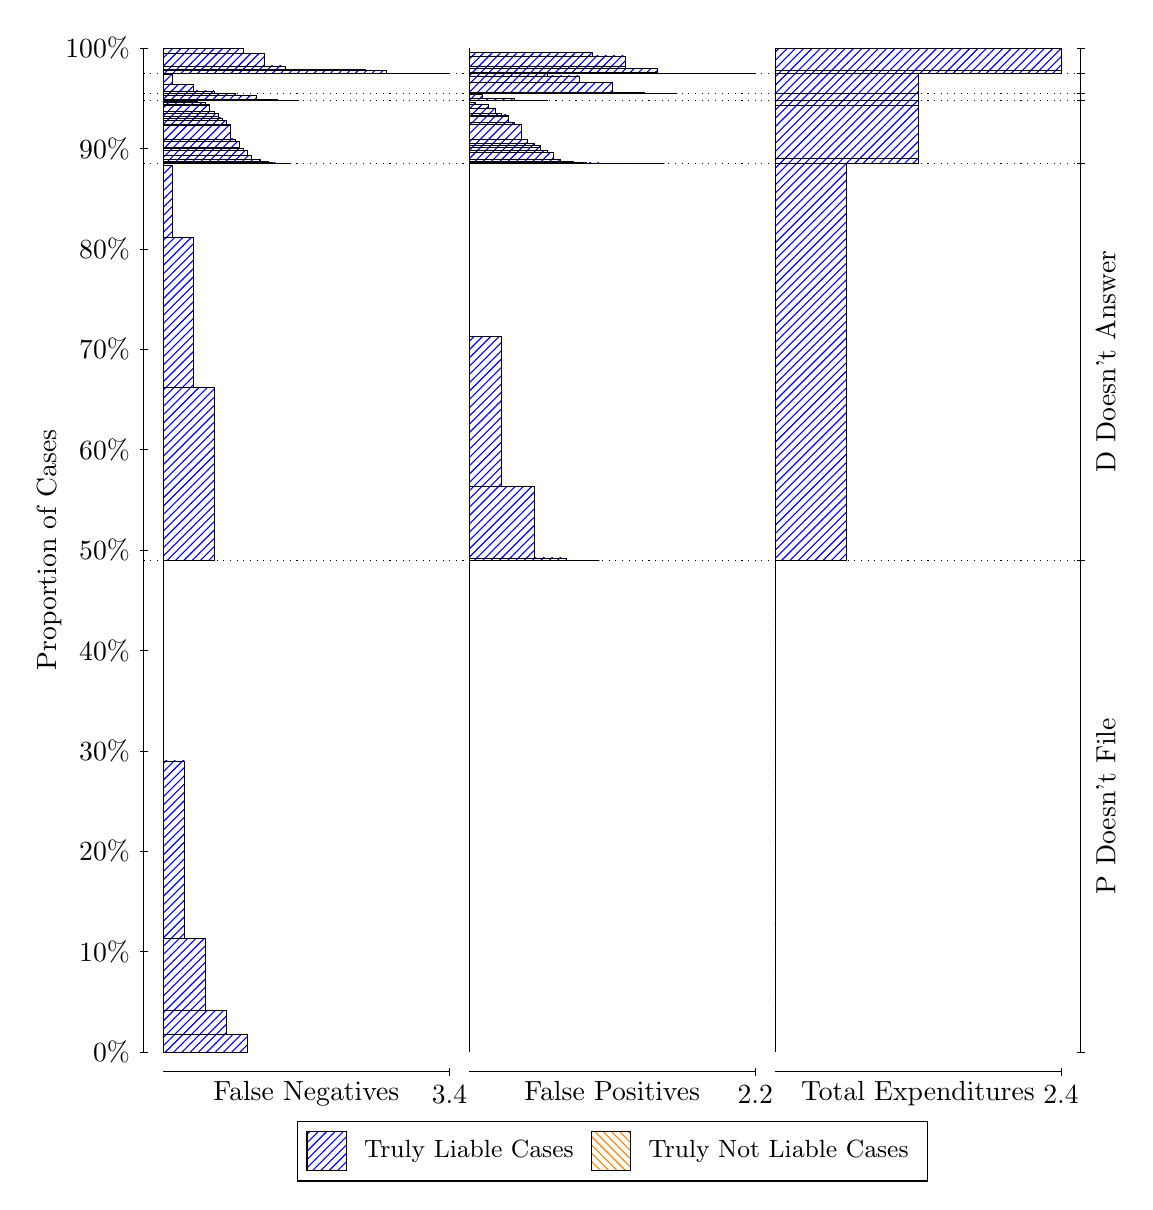
\begin{tikzpicture}
\draw[black, very thin] (1.5,1.75) -- (1.5,14.5);
\node[rotate=90, anchor=center] at (0.3, 8.125) {Proportion of Cases};
\draw[black, very thin] (1.45,1.75) -- (1.55,1.75);
\node[anchor=east] at (1.45, 1.75) {0\%};
\draw[black, very thin] (1.45,3.025) -- (1.55,3.025);
\node[anchor=east] at (1.45, 3.025) {10\%};
\draw[black, very thin] (1.45,4.3) -- (1.55,4.3);
\node[anchor=east] at (1.45, 4.3) {20\%};
\draw[black, very thin] (1.45,5.575) -- (1.55,5.575);
\node[anchor=east] at (1.45, 5.575) {30\%};
\draw[black, very thin] (1.45,6.85) -- (1.55,6.85);
\node[anchor=east] at (1.45, 6.85) {40\%};
\draw[black, very thin] (1.45,8.125) -- (1.55,8.125);
\node[anchor=east] at (1.45, 8.125) {50\%};
\draw[black, very thin] (1.45,9.4) -- (1.55,9.4);
\node[anchor=east] at (1.45, 9.4) {60\%};
\draw[black, very thin] (1.45,10.675) -- (1.55,10.675);
\node[anchor=east] at (1.45, 10.675) {70\%};
\draw[black, very thin] (1.45,11.95) -- (1.55,11.95);
\node[anchor=east] at (1.45, 11.95) {80\%};
\draw[black, very thin] (1.45,13.225) -- (1.55,13.225);
\node[anchor=east] at (1.45, 13.225) {90\%};
\draw[black, very thin] (1.45,14.5) -- (1.55,14.5);
\node[anchor=east] at (1.45, 14.5) {100\%};

\draw[black, very thin] (13.4,1.75) -- (13.4,14.5);
\draw[black, very thin] (13.35,1.75) -- (13.45,1.75);
\node[anchor=west] at (13.35, 1.75) {};
\draw[black, very thin] (13.35,7.9952) -- (13.45,7.9952);
\node[anchor=west] at (13.35, 7.9952) {};
\draw[black, very thin] (13.35,13.038) -- (13.45,13.038);
\node[anchor=west] at (13.35, 13.038) {};
\draw[black, very thin] (13.35,13.833) -- (13.45,13.833);
\node[anchor=west] at (13.35, 13.833) {};
\draw[black, very thin] (13.35,13.927) -- (13.45,13.927);
\node[anchor=west] at (13.35, 13.927) {};
\draw[black, very thin] (13.35,14.175) -- (13.45,14.175);
\node[anchor=west] at (13.35, 14.175) {};
\draw[black, very thin] (13.35,14.5) -- (13.45,14.5);
\node[anchor=west] at (13.35, 14.5) {};

\draw[black, very thin, pattern color=blue, pattern=north east lines] (1.75,1.75) rectangle (2.8186,1.9782);
\draw[black, very thin, pattern color=blue, pattern=north east lines] (1.75,1.9782) rectangle (2.5515,2.2818);
\draw[black, very thin, pattern color=blue, pattern=north east lines] (1.75,2.2818) rectangle (2.2843,3.1942);
\draw[black, very thin, pattern color=blue, pattern=north east lines] (1.75,3.1942) rectangle (2.0172,5.4482);
\draw[black, very thin, pattern color=orange, pattern=north west lines] (1.75,5.4482) rectangle (1.75,5.4482);
\draw[black, very thin, pattern color=blue, pattern=north east lines] (1.75,5.4482) rectangle (1.75,7.9952);
\draw[black, very thin, pattern color=blue, pattern=north east lines] (1.75,7.9952) rectangle (2.3912,10.194);
\draw[black, very thin, pattern color=blue, pattern=north east lines] (1.75,10.194) rectangle (2.124,12.1);
\draw[black, very thin, pattern color=blue, pattern=north east lines] (1.75,12.1) rectangle (1.8569,13.009);
\draw[black, very thin, pattern color=orange, pattern=north west lines] (1.75,13.009) rectangle (1.75,13.009);
\draw[black, very thin, pattern color=blue, pattern=north east lines] (1.75,13.009) rectangle (1.75,13.038);
\draw[black, very thin, pattern color=blue, pattern=north east lines] (1.75,13.038) rectangle (3.3529,13.039);
\draw[black, very thin, pattern color=blue, pattern=north east lines] (1.75,13.039) rectangle (3.2461,13.041);
\draw[black, very thin, pattern color=blue, pattern=north east lines] (1.75,13.041) rectangle (3.1392,13.045);
\draw[black, very thin, pattern color=blue, pattern=north east lines] (1.75,13.045) rectangle (3.0858,13.059);
\draw[black, very thin, pattern color=blue, pattern=north east lines] (1.75,13.059) rectangle (3.0324,13.062);
\draw[black, very thin, pattern color=blue, pattern=north east lines] (1.75,13.062) rectangle (2.9789,13.081);
\draw[black, very thin, pattern color=blue, pattern=north east lines] (1.75,13.081) rectangle (2.9255,13.089);
\draw[black, very thin, pattern color=blue, pattern=north east lines] (1.75,13.089) rectangle (2.8721,13.133);
\draw[black, very thin, pattern color=blue, pattern=north east lines] (1.75,13.133) rectangle (2.8186,13.198);
\draw[black, very thin, pattern color=blue, pattern=north east lines] (1.75,13.198) rectangle (2.7652,13.222);
\draw[black, very thin, pattern color=blue, pattern=north east lines] (1.75,13.222) rectangle (2.7118,13.234);
\draw[black, very thin, pattern color=blue, pattern=north east lines] (1.75,13.234) rectangle (2.7118,13.317);
\draw[black, very thin, pattern color=blue, pattern=north east lines] (1.75,13.317) rectangle (2.6583,13.346);
\draw[black, very thin, pattern color=blue, pattern=north east lines] (1.75,13.346) rectangle (2.6049,13.525);
\draw[black, very thin, pattern color=blue, pattern=north east lines] (1.75,13.525) rectangle (2.6049,13.533);
\draw[black, very thin, pattern color=blue, pattern=north east lines] (1.75,13.533) rectangle (2.5515,13.578);
\draw[black, very thin, pattern color=blue, pattern=north east lines] (1.75,13.578) rectangle (2.498,13.612);
\draw[black, very thin, pattern color=blue, pattern=north east lines] (1.75,13.612) rectangle (2.4446,13.63);
\draw[black, very thin, pattern color=blue, pattern=north east lines] (1.75,13.63) rectangle (2.4446,13.668);
\draw[black, very thin, pattern color=blue, pattern=north east lines] (1.75,13.668) rectangle (2.3912,13.696);
\draw[black, very thin, pattern color=blue, pattern=north east lines] (1.75,13.696) rectangle (2.3377,13.776);
\draw[black, very thin, pattern color=blue, pattern=north east lines] (1.75,13.776) rectangle (2.3377,13.788);
\draw[black, very thin, pattern color=blue, pattern=north east lines] (1.75,13.788) rectangle (2.2843,13.808);
\draw[black, very thin, pattern color=blue, pattern=north east lines] (1.75,13.808) rectangle (2.2309,13.808);
\draw[black, very thin, pattern color=blue, pattern=north east lines] (1.75,13.808) rectangle (2.2309,13.814);
\draw[black, very thin, pattern color=blue, pattern=north east lines] (1.75,13.814) rectangle (2.1775,13.822);
\draw[black, very thin, pattern color=blue, pattern=north east lines] (1.75,13.822) rectangle (2.1775,13.823);
\draw[black, very thin, pattern color=blue, pattern=north east lines] (1.75,13.823) rectangle (2.124,13.824);
\draw[black, very thin, pattern color=blue, pattern=north east lines] (1.75,13.824) rectangle (2.0706,13.825);
\draw[black, very thin, pattern color=blue, pattern=north east lines] (1.75,13.825) rectangle (2.0706,13.83);
\draw[black, very thin, pattern color=blue, pattern=north east lines] (1.75,13.83) rectangle (2.0172,13.831);
\draw[black, very thin, pattern color=blue, pattern=north east lines] (1.75,13.831) rectangle (1.9637,13.831);
\draw[black, very thin, pattern color=blue, pattern=north east lines] (1.75,13.831) rectangle (1.9637,13.833);
\draw[black, very thin, pattern color=blue, pattern=north east lines] (1.75,13.833) rectangle (1.9103,13.833);
\draw[black, very thin, pattern color=blue, pattern=north east lines] (1.75,13.833) rectangle (1.8569,13.833);
\draw[black, very thin, pattern color=blue, pattern=north east lines] (1.75,13.833) rectangle (1.8034,13.833);
\draw[black, very thin, pattern color=orange, pattern=north west lines] (1.75,13.833) rectangle (1.75,13.833);
\draw[black, very thin, pattern color=blue, pattern=north east lines] (1.75,13.833) rectangle (1.75,13.833);
\draw[black, very thin, pattern color=blue, pattern=north east lines] (1.75,13.833) rectangle (3.4598,13.836);
\draw[black, very thin, pattern color=blue, pattern=north east lines] (1.75,13.836) rectangle (3.1926,13.846);
\draw[black, very thin, pattern color=blue, pattern=north east lines] (1.75,13.846) rectangle (2.9255,13.897);
\draw[black, very thin, pattern color=blue, pattern=north east lines] (1.75,13.897) rectangle (2.6583,13.926);
\draw[black, very thin, pattern color=blue, pattern=north east lines] (1.75,13.926) rectangle (2.3912,13.927);
\draw[black, very thin, pattern color=orange, pattern=north west lines] (1.75,13.927) rectangle (1.75,13.927);
\draw[black, very thin, pattern color=blue, pattern=north east lines] (1.75,13.927) rectangle (2.3912,13.956);
\draw[black, very thin, pattern color=blue, pattern=north east lines] (1.75,13.956) rectangle (2.124,14.042);
\draw[black, very thin, pattern color=blue, pattern=north east lines] (1.75,14.042) rectangle (1.8569,14.17);
\draw[black, very thin, pattern color=orange, pattern=north west lines] (1.75,14.17) rectangle (1.75,14.17);
\draw[black, very thin, pattern color=blue, pattern=north east lines] (1.75,14.17) rectangle (1.75,14.175);
\draw[black, very thin, pattern color=blue, pattern=north east lines] (1.75,14.175) rectangle (5.3833,14.175);
\draw[black, very thin, pattern color=blue, pattern=north east lines] (1.75,14.175) rectangle (5.1162,14.175);
\draw[black, very thin, pattern color=blue, pattern=north east lines] (1.75,14.175) rectangle (4.849,14.179);
\draw[black, very thin, pattern color=blue, pattern=north east lines] (1.75,14.179) rectangle (4.5819,14.213);
\draw[black, very thin, pattern color=blue, pattern=north east lines] (1.75,14.213) rectangle (4.3147,14.228);
\draw[black, very thin, pattern color=blue, pattern=north east lines] (1.75,14.228) rectangle (4.0475,14.228);
\draw[black, very thin, pattern color=blue, pattern=north east lines] (1.75,14.228) rectangle (3.8338,14.228);
\draw[black, very thin, pattern color=blue, pattern=north east lines] (1.75,14.228) rectangle (3.7804,14.228);
\draw[black, very thin, pattern color=blue, pattern=north east lines] (1.75,14.228) rectangle (3.5667,14.229);
\draw[black, very thin, pattern color=blue, pattern=north east lines] (1.75,14.229) rectangle (3.2995,14.273);
\draw[black, very thin, pattern color=blue, pattern=north east lines] (1.75,14.273) rectangle (3.0324,14.429);
\draw[black, very thin, pattern color=blue, pattern=north east lines] (1.75,14.429) rectangle (2.7652,14.495);
\draw[black, very thin, pattern color=blue, pattern=north east lines] (1.75,14.495) rectangle (2.498,14.5);
\draw[black, very thin, pattern color=blue, pattern=north east lines] (1.75,14.5) rectangle (2.2309,14.5);
\draw[black, very thin, pattern color=blue, pattern=north east lines] (1.75,14.5) rectangle (1.9637,14.5);
\draw[black, very thin, pattern color=orange, pattern=north west lines] (1.75,14.5) rectangle (1.75,14.5);
\draw[black, very thin, pattern color=orange, pattern=north west lines] (5.6333,1.75) rectangle (5.6333,1.75);
\draw[black, very thin, pattern color=blue, pattern=north east lines] (5.6333,1.75) rectangle (5.6333,7.9952);
\draw[black, very thin, pattern color=orange, pattern=north west lines] (5.6333,7.9952) rectangle (7.2848,7.9952);
\draw[black, very thin, pattern color=blue, pattern=north east lines] (5.6333,7.9952) rectangle (7.2848,7.9952);
\draw[black, very thin, pattern color=blue, pattern=north east lines] (5.6333,7.9952) rectangle (6.872,8.024);
\draw[black, very thin, pattern color=blue, pattern=north east lines] (5.6333,8.024) rectangle (6.4591,8.9334);
\draw[black, very thin, pattern color=blue, pattern=north east lines] (5.6333,8.9334) rectangle (6.0462,10.84);
\draw[black, very thin, pattern color=blue, pattern=north east lines] (5.6333,10.84) rectangle (5.6333,13.038);
\draw[black, very thin, pattern color=orange, pattern=north west lines] (5.6333,13.038) rectangle (8.1106,13.038);
\draw[black, very thin, pattern color=blue, pattern=north east lines] (5.6333,13.038) rectangle (8.1106,13.038);
\draw[black, very thin, pattern color=orange, pattern=north west lines] (5.6333,13.038) rectangle (7.9455,13.038);
\draw[black, very thin, pattern color=blue, pattern=north east lines] (5.6333,13.038) rectangle (7.9455,13.038);
\draw[black, very thin, pattern color=orange, pattern=north west lines] (5.6333,13.038) rectangle (7.7803,13.038);
\draw[black, very thin, pattern color=blue, pattern=north east lines] (5.6333,13.038) rectangle (7.7803,13.038);
\draw[black, very thin, pattern color=blue, pattern=north east lines] (5.6333,13.038) rectangle (7.6977,13.038);
\draw[black, very thin, pattern color=orange, pattern=north west lines] (5.6333,13.038) rectangle (7.6152,13.038);
\draw[black, very thin, pattern color=blue, pattern=north east lines] (5.6333,13.038) rectangle (7.6152,13.038);
\draw[black, very thin, pattern color=blue, pattern=north east lines] (5.6333,13.038) rectangle (7.5326,13.038);
\draw[black, very thin, pattern color=orange, pattern=north west lines] (5.6333,13.038) rectangle (7.45,13.038);
\draw[black, very thin, pattern color=blue, pattern=north east lines] (5.6333,13.038) rectangle (7.45,13.038);
\draw[black, very thin, pattern color=blue, pattern=north east lines] (5.6333,13.038) rectangle (7.3674,13.038);
\draw[black, very thin, pattern color=orange, pattern=north west lines] (5.6333,13.038) rectangle (7.2848,13.038);
\draw[black, very thin, pattern color=blue, pattern=north east lines] (5.6333,13.038) rectangle (7.2848,13.041);
\draw[black, very thin, pattern color=blue, pattern=north east lines] (5.6333,13.041) rectangle (7.2023,13.042);
\draw[black, very thin, pattern color=orange, pattern=north west lines] (5.6333,13.042) rectangle (7.1197,13.042);
\draw[black, very thin, pattern color=blue, pattern=north east lines] (5.6333,13.042) rectangle (7.1197,13.048);
\draw[black, very thin, pattern color=blue, pattern=north east lines] (5.6333,13.048) rectangle (7.0371,13.049);
\draw[black, very thin, pattern color=orange, pattern=north west lines] (5.6333,13.049) rectangle (6.9545,13.049);
\draw[black, very thin, pattern color=blue, pattern=north east lines] (5.6333,13.049) rectangle (6.9545,13.049);
\draw[black, very thin, pattern color=blue, pattern=north east lines] (5.6333,13.049) rectangle (6.9545,13.057);
\draw[black, very thin, pattern color=blue, pattern=north east lines] (5.6333,13.057) rectangle (6.872,13.063);
\draw[black, very thin, pattern color=orange, pattern=north west lines] (5.6333,13.063) rectangle (6.7894,13.063);
\draw[black, very thin, pattern color=blue, pattern=north east lines] (5.6333,13.063) rectangle (6.7894,13.083);
\draw[black, very thin, pattern color=blue, pattern=north east lines] (5.6333,13.083) rectangle (6.7068,13.176);
\draw[black, very thin, pattern color=blue, pattern=north east lines] (5.6333,13.176) rectangle (6.6242,13.203);
\draw[black, very thin, pattern color=blue, pattern=north east lines] (5.6333,13.203) rectangle (6.5417,13.241);
\draw[black, very thin, pattern color=blue, pattern=north east lines] (5.6333,13.241) rectangle (6.5417,13.26);
\draw[black, very thin, pattern color=blue, pattern=north east lines] (5.6333,13.26) rectangle (6.4591,13.293);
\draw[black, very thin, pattern color=blue, pattern=north east lines] (5.6333,13.293) rectangle (6.3765,13.339);
\draw[black, very thin, pattern color=blue, pattern=north east lines] (5.6333,13.339) rectangle (6.2939,13.526);
\draw[black, very thin, pattern color=blue, pattern=north east lines] (5.6333,13.526) rectangle (6.2114,13.554);
\draw[black, very thin, pattern color=blue, pattern=north east lines] (5.6333,13.554) rectangle (6.1288,13.638);
\draw[black, very thin, pattern color=blue, pattern=north east lines] (5.6333,13.638) rectangle (6.1288,13.65);
\draw[black, very thin, pattern color=blue, pattern=north east lines] (5.6333,13.65) rectangle (6.0462,13.674);
\draw[black, very thin, pattern color=blue, pattern=north east lines] (5.6333,13.674) rectangle (5.9636,13.739);
\draw[black, very thin, pattern color=blue, pattern=north east lines] (5.6333,13.739) rectangle (5.8811,13.782);
\draw[black, very thin, pattern color=blue, pattern=north east lines] (5.6333,13.782) rectangle (5.7985,13.79);
\draw[black, very thin, pattern color=blue, pattern=north east lines] (5.6333,13.79) rectangle (5.7159,13.809);
\draw[black, very thin, pattern color=blue, pattern=north east lines] (5.6333,13.809) rectangle (5.6333,13.833);
\draw[black, very thin, pattern color=orange, pattern=north west lines] (5.6333,13.833) rectangle (6.6242,13.833);
\draw[black, very thin, pattern color=blue, pattern=north east lines] (5.6333,13.833) rectangle (6.6242,13.834);
\draw[black, very thin, pattern color=blue, pattern=north east lines] (5.6333,13.834) rectangle (6.2114,13.863);
\draw[black, very thin, pattern color=blue, pattern=north east lines] (5.6333,13.863) rectangle (5.7985,13.914);
\draw[black, very thin, pattern color=blue, pattern=north east lines] (5.6333,13.914) rectangle (5.6333,13.927);
\draw[black, very thin, pattern color=orange, pattern=north west lines] (5.6333,13.927) rectangle (8.2758,13.927);
\draw[black, very thin, pattern color=blue, pattern=north east lines] (5.6333,13.927) rectangle (8.2758,13.927);
\draw[black, very thin, pattern color=blue, pattern=north east lines] (5.6333,13.927) rectangle (7.8629,13.932);
\draw[black, very thin, pattern color=blue, pattern=north east lines] (5.6333,13.932) rectangle (7.45,14.06);
\draw[black, very thin, pattern color=blue, pattern=north east lines] (5.6333,14.06) rectangle (7.0371,14.145);
\draw[black, very thin, pattern color=blue, pattern=north east lines] (5.6333,14.145) rectangle (6.6242,14.175);
\draw[black, very thin, pattern color=orange, pattern=north west lines] (5.6333,14.175) rectangle (9.2667,14.175);
\draw[black, very thin, pattern color=blue, pattern=north east lines] (5.6333,14.175) rectangle (9.2667,14.175);
\draw[black, very thin, pattern color=blue, pattern=north east lines] (5.6333,14.175) rectangle (8.8538,14.175);
\draw[black, very thin, pattern color=orange, pattern=north west lines] (5.6333,14.175) rectangle (8.8538,14.175);
\draw[black, very thin, pattern color=blue, pattern=north east lines] (5.6333,14.175) rectangle (8.8538,14.175);
\draw[black, very thin, pattern color=blue, pattern=north east lines] (5.6333,14.175) rectangle (8.4409,14.178);
\draw[black, very thin, pattern color=orange, pattern=north west lines] (5.6333,14.178) rectangle (8.4409,14.178);
\draw[black, very thin, pattern color=blue, pattern=north east lines] (5.6333,14.178) rectangle (8.4409,14.18);
\draw[black, very thin, pattern color=blue, pattern=north east lines] (5.6333,14.18) rectangle (8.028,14.194);
\draw[black, very thin, pattern color=orange, pattern=north west lines] (5.6333,14.194) rectangle (8.028,14.194);
\draw[black, very thin, pattern color=blue, pattern=north east lines] (5.6333,14.194) rectangle (8.028,14.246);
\draw[black, very thin, pattern color=blue, pattern=north east lines] (5.6333,14.246) rectangle (7.6152,14.273);
\draw[black, very thin, pattern color=blue, pattern=north east lines] (5.6333,14.273) rectangle (7.6152,14.401);
\draw[black, very thin, pattern color=blue, pattern=north east lines] (5.6333,14.401) rectangle (7.2023,14.446);
\draw[black, very thin, pattern color=blue, pattern=north east lines] (5.6333,14.446) rectangle (6.7894,14.447);
\draw[black, very thin, pattern color=orange, pattern=north west lines] (5.6333,14.447) rectangle (6.4591,14.447);
\draw[black, very thin, pattern color=blue, pattern=north east lines] (5.6333,14.447) rectangle (6.4591,14.447);
\draw[black, very thin, pattern color=blue, pattern=north east lines] (5.6333,14.447) rectangle (6.3765,14.447);
\draw[black, very thin, pattern color=orange, pattern=north west lines] (5.6333,14.447) rectangle (6.0462,14.447);
\draw[black, very thin, pattern color=blue, pattern=north east lines] (5.6333,14.447) rectangle (6.0462,14.447);
\draw[black, very thin, pattern color=orange, pattern=north west lines] (5.6333,14.447) rectangle (5.6333,14.447);
\draw[black, very thin, pattern color=blue, pattern=north east lines] (5.6333,14.447) rectangle (5.6333,14.5);
\draw[black, very thin, pattern color=orange, pattern=north west lines] (9.5167,1.75) rectangle (9.5167,1.75);
\draw[black, very thin, pattern color=blue, pattern=north east lines] (9.5167,1.75) rectangle (9.5167,7.9952);
\draw[black, very thin, pattern color=orange, pattern=north west lines] (9.5167,7.9952) rectangle (10.425,7.9952);
\draw[black, very thin, pattern color=blue, pattern=north east lines] (9.5167,7.9952) rectangle (10.425,13.038);
\draw[black, very thin, pattern color=orange, pattern=north west lines] (9.5167,13.038) rectangle (11.333,13.038);
\draw[black, very thin, pattern color=blue, pattern=north east lines] (9.5167,13.038) rectangle (11.333,13.103);
\draw[black, very thin, pattern color=orange, pattern=north west lines] (9.5167,13.103) rectangle (11.333,13.103);
\draw[black, very thin, pattern color=blue, pattern=north east lines] (9.5167,13.103) rectangle (11.333,13.769);
\draw[black, very thin, pattern color=orange, pattern=north west lines] (9.5167,13.769) rectangle (11.333,13.769);
\draw[black, very thin, pattern color=blue, pattern=north east lines] (9.5167,13.769) rectangle (11.333,13.833);
\draw[black, very thin, pattern color=orange, pattern=north west lines] (9.5167,13.833) rectangle (11.333,13.833);
\draw[black, very thin, pattern color=blue, pattern=north east lines] (9.5167,13.833) rectangle (11.333,13.927);
\draw[black, very thin, pattern color=orange, pattern=north west lines] (9.5167,13.927) rectangle (11.333,13.927);
\draw[black, very thin, pattern color=blue, pattern=north east lines] (9.5167,13.927) rectangle (11.333,14.175);
\draw[black, very thin, pattern color=orange, pattern=north west lines] (9.5167,14.175) rectangle (13.15,14.175);
\draw[black, very thin, pattern color=blue, pattern=north east lines] (9.5167,14.175) rectangle (13.15,14.218);
\draw[black, very thin, pattern color=orange, pattern=north west lines] (9.5167,14.218) rectangle (13.15,14.218);
\draw[black, very thin, pattern color=blue, pattern=north east lines] (9.5167,14.218) rectangle (13.15,14.5);
\draw[black, dotted] (1.5,7.9952) -- (13.4,7.9952);
\draw[black, dotted] (1.5,13.038) -- (13.4,13.038);
\draw[black, dotted] (1.5,13.833) -- (13.4,13.833);
\draw[black, dotted] (1.5,13.927) -- (13.4,13.927);
\draw[black, dotted] (1.5,14.175) -- (13.4,14.175);
\draw[black, very thin] (1.75,1.5) -- (5.3833,1.5);
\node[anchor=north] at (3.5667, 1.5) {False Negatives};
\draw[black, very thin] (5.3833,1.45) -- (5.3833,1.55);
\node[anchor=north] at (5.3833, 1.45) {3.4};

\draw[black, very thin] (5.6333,1.5) -- (9.2667,1.5);
\node[anchor=north] at (7.45, 1.5) {False Positives};
\draw[black, very thin] (9.2667,1.45) -- (9.2667,1.55);
\node[anchor=north] at (9.2667, 1.45) {2.2};

\draw[black, very thin] (9.5167,1.5) -- (13.15,1.5);
\node[anchor=north] at (11.333, 1.5) {Total Expenditures};
\draw[black, very thin] (13.15,1.45) -- (13.15,1.55);
\node[anchor=north] at (13.15, 1.45) {2.4};

\node[black, centered, rotate=90] at (13.72, 4.8726) {P Doesn't File};
\node[black, centered, rotate=90] at (13.72, 10.517) {D Doesn't Answer};





\draw (7.449999999999999,1.5) node[draw=none] (baseCoordinate) {};
\begin{scope}[align=center]
        \matrix[scale=0.5, draw=black, below=0.5cm of baseCoordinate, nodes={draw}, column sep=0.1cm]{
            \node[rectangle, draw, minimum width=0.5cm, minimum height=0.5cm, pattern=north east lines, pattern color=blue] {}; &
            \node[draw=none, font=\small] (B) {Truly Liable Cases}; &
            \node[rectangle, draw, minimum width=0.5cm, minimum height=0.5cm, pattern=north west lines, pattern color=orange] {}; &
            \node[draw=none, font=\small] (B) {Truly Not Liable Cases}; \\
            };
\end{scope}

\end{tikzpicture}
\end{document}